%!TEX root=../Emile.tex
\section[Exposition]{Exposition}

\subsection[Tilly]{Tilly: Staatsgenese als organisiertes Verbrechen}

\epigraph{
	``Homo homini lupus.''\\*
	\emph{\parencite{Hobbes-1651-aa}}
}

Bei genauerem Hinschauen erkennt man, dass das Kursthema voraussetzt, dass Demokratie überhaupt erstrebenswert ist.
Da kollektiv verbindliche Entscheidungen einer Demokratie inhärent sind, braucht man einen Staat, der diese unter Zwang durchsetzt.
Die Entstehung von Staaten ist das Thema Charles Tillys.
Staaten definiert er als die Kontrolle der physischen Gewalt über ein Volk auf einem zusammenhängenden Territorium:

\begin{quote}
	``national states: relatively centralized, differentiated organizations the officials of which more or less successfully claim control over the chief concentrated means of violence within a population inhabiting a large, contiguous territory.''\\*
	\parencite[170]{Tilly-1985-aa}.
\end{quote}


\paragraph{Wie entsteht ein Staat?}

Nach Tilly ist die Entwicklung eines Staates immer mit kriegerischen und gewaltvollen Handlungen verbunden.
Er geht sogar so weit zu behaupten, dass Gewalt notwendig für die Entwicklung eines Staates sei.
Der Ausgangspunkt für die Entwicklung eines Staates ist die Monopolisierung von Gewalt und Macht: ``governments organize and, wherever possible, monopolize violence'' \parencite[171]{Tilly-1985-aa}.
\citeauthor{Tilly-1985-aa} sagt, dass in der vor-staatlichen Zeit mehrere gewaltausübende Parteien konkurrierten.
Ähnlich einem \citeauthor{Hobbes-1651-aa}chen Urzustands, führt in diesem Wettbewerb jede Partei Krieg gegen jede.
Dabei ist jene Person oder Gruppe im Vorteil, der es gelingt, positive Skalenerträge zu erzielen, also zu \emph{fallenden} Grenzkosten \emph{mehr} Gewalt (oder deren glaubhafte Androhung) zu produzieren.
Positive Skalenerträge entstehen, wenn die Kosten für die jeweils \emph{nächste} produzierte Einheit Gewalt sinken.
Tilly's konkurrierende Gewaltunternehmer versuchen sich durch technische oder organisatorische Innovationen einen Vorteil über die anderen Parteien zu verschaffen, um sich innerhalb eines geografischen Gebietes durchzusetzen \parencite[vgl.][173]{Tilly-1985-aa}.

\begin{dsafigure}
	\begin{center}
	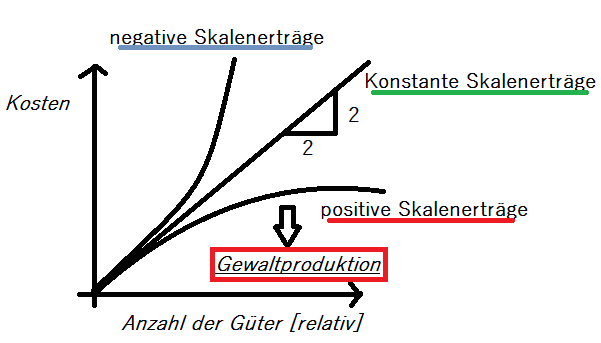
\includegraphics[width=0.9\columnwidth]{img/Skalenertraege.png}
	\caption{Positive Skalenerträge}
	\label{fig:skalenertraege}
	\end{center}
\end{dsafigure}

Für die herrschende Partei ist das insofern ein Vorteil, alsdass sie mit geringeren Kosten effizienter Gewalt ``produzieren'' kann.
Positive Skalenerträge kommen vor allem durch technische und organisatorische Innovationen zustande.
So ist beispielsweise bei niedrig entwickelten Waffen (wie Keulen) kaum ein solcher Vorteil erkennbar.
Es kostet einen bestimmten Geldbetrag, eine Keule herzustellen, die eine Person ausschalten kann.
Dieser Betrag bleibt auch bei den nächsten tausend produzierten Keulen ungefähr gleich.
Dadurch ergibt sich kein großer Vorteil.

Anders verhält es sich bei höher entwickelten Waffen wie der Wasserstoffbombe.
Hat diese bei einem Ertrag von mehreren Millionen Menschen, die auf einmal ausgeschaltet werden können, bei der ersten Herstellung noch extrem große Produktionskosten, so werden diese bei den nächsten produzierten Bomben deutlich kleiner.
Für die herrschende Partei stellt dies einen militärischen Vorteil dar.
Er kann mit höherer Produktion deutlich höhere Erträge bei gleichen Kosten erzielen und so die Konkurrenten ausschalten.

Positive Skalenerträge können damit erklären, wie aus vielen, relativ kleinen konkurrierenden Gewaltunternehmern (``Schutzgelderpressern''), effektive Monopolisten (``(National)staaten'') entstehen konnten.

Dieses Handeln ist entscheidend für die Entwicklung eines Staates, denn es zeigt, dass ein Staat nicht etwa infolge von friedlicher Zusammenarbeit der Menschen entsteht, sondern dieser materialistischen Theorie folgend an Machtkämpfe, Ausbeutung und Krieg gebunden ist: ``war making likewise led to state making'' \parencite[183]{Tilly-1985-aa}.

Durch sein Gewaltmonopol hat die herrschende Gruppe die Möglichkeit, von seinem Volk Tribute (Steuern) einzufordern und im Gegenzug \emph{Sicherheit} anzubieten: ``governments are in the business of selling protection'' \parencite[175]{Tilly-1985-aa}.
Allerdings funktioniert dies nur durch anhaltende Gewaltpräsenz und durch Drohungen des Herrschers.

\citeauthor{Tilly-1985-aa} betont dabei den paradox scheinenden Kontrast: der Staat droht mit Gewalt und schützt gleichzeitig vor ihr.


\paragraph{Durch welche Handlungen definiert sich ein Staat?}

Nachdem der Staat durch \emph{Unterwerfung} das Machtmonopol installiert hat \parencite[vgl.][175]{Tilly-1985-aa}, \emph{definiert} er sich durch das sogenannte \emph{Gewaltmonopol}: ``the authority's monopoly of force'' \parencite[vgl.][172]{Tilly-1985-aa}.
In Tillys Verständnis kann man dies als das Alleinrecht auf Sicherheit und Ordnung auf einem bestimmten Gebiet verstehen: ``governments claim to provide protection'' \parencite[vgl.][172]{Tilly-1985-aa}.
Andere Leistungen wie z.B.\ eine Krankenversicherung, die Deutsche Schülerakademie oder eine allgemeine Schulpflicht sind nicht Teil von Tillys Staatsverständnis \parencite[vgl.][181]{Tilly-1985-aa} ––– diese oder andere öffentliche Güter können aber dieser materialistischen Theorie folgend nur vor dem Hintergrund eines effektiven Gewaltmonopols produziert werden.